% !TEX TS-program = pdflatex
% !TEX encoding = UTF-8 Unicode

% This is a simple template for a LaTeX document using the "article" class.
% See "book", "report", "letter" for other types of document.

\documentclass[11pt,a4paper,titlepage=firstiscover,headsepline,bibtotoc]{scrartcl} % use larger type; default would be 10pt

\usepackage[utf8]{inputenc} % set input encoding (not needed with XeLaTeX)
\usepackage[T1]{fontenc} % maps glyphs to dictonary characters, needed for seperation

%%% Examples of Article customizations
% These packages are optional, depending whether you want the features they provide.
% See the LaTeX Companion or other references for full information.

%%% PAGE DIMENSIONS
\usepackage{geometry} % to change the page dimensions
%\geometry{a4paper} % or letterpaper (US) or a5paper or....
\geometry{top=3.5cm,bottom=3.5cm} % for example, change the margins to 2 inches all round
% \geometry{landscape} % set up the page for landscape
%   read geometry.pdf for detailed page layout information

\usepackage{tocstyle}

% \usepackage[parfill]{parskip} % Activate to begin paragraphs with an empty line rather than an indent

%%% PACKAGES
%\usepackage{booktabs} % for much better looking tables
\usepackage{tabularx}  % for tables with variable width
%\usepackage{array} % for better arrays (eg matrices) in maths

%\usepackage{subfig} % make it possible to include more than one captioned figure/table in a single float
% These packages are all incorporated in the memoir class to one degree or another...
\usepackage[ngerman]{babel}
\usepackage{eurosym} %for euro symbol via \euro
%\usepackage{blindtext}
%\usepackage{pifont} %for symbols (i.e. arrows)
%\usepackage{showframe} %shows the margins
\usepackage{hhline} % more flexible hlines
\usepackage{graphicx}


\usepackage[colorlinks,linkcolor=blue,pdftex]{hyperref} % package for hyperlinks with \url
% hyperlink color definitions
%\hypersetup{citecolor=DeepPink4}
%\hypersetup{linkcolor=DarkRed}
%\hypersetup{urlcolor=DarkBlue} 

%\usepackage[svgnames]{xcolor}
%\usepackage[anythingbreaks]{breakurl}
\usepackage{listings}
\lstset{ %
%basicstyle=\sfdefault,        % the size of the fonts that are used for the code
%breakatwhitespace=false,         % sets if automatic breaks should only happen at whitespace
breaklines=true,                 % sets automatic line breaking
%commentstyle=\color{mygreen},    % comment style
%deletekeywords={...},            % if you want to delete keywords from the given language
%escapeinside={\%*}{*)},          % if you want to add LaTeX within your code
%extendedchars=true,              % lets you use non-ASCII characters; for 8-bits encodings only, does not work with UTF-8
frame=single,                    % adds a frame around the code
keepspaces=true,                 % keeps spaces in text, useful for keeping indentation of code (possibly needs columns=flexible)
%keywordstyle=\color{mygreen},       % keyword style
%morekeywords={*,...},            % if you want to add more keywords to the set
numbers=none,                    % where to put the line-numbers; possible values are (none, left, right)
%numbersep=5pt,                   % how far the line-numbers are from the code
%numberstyle=\tiny\color{mygray}, % the style that is used for the line-numbers
%rulecolor=\color{black},         % if not set, the frame-color may be changed on line-breaks within not-black text (e.g. comments (green here))
%showspaces=false,                % show spaces everywhere adding particular underscores; it overrides 'showstringspaces'
%showstringspaces=false,          % underline spaces within strings only
%showtabs=false,                  % show tabs within strings adding particular underscores
%stepnumber=2,                    % the step between two line-numbers. If it's 1, each line will be numbered
%stringstyle=\ttfamily\color{red},     % string literal style
%tabsize=2,                       % sets default tabsize to 2 spaces
%title=\lstname                   % show the filename of files included with \lstinputlisting; also try caption instead of title
}

\newcommand{\hilight}[1]{\colorbox{yellow}{#1}} %command for magic marker highlighting
%   (from http://pleasemakeanote.blogspot.de/2009/08/how-to-highlight-text-in-latex.html)
\newcommand{\mcc}[2]{\multicolumn{#1}{|c|}{#2}} %multirows over X rows in tabularx

%%% HEADERS & FOOTERS
\usepackage[automark]{scrlayer-scrpage} %header and footer definitions
\setkomafont{pageheadfoot}{\normalfont\normalcolor} %um kursiv abzuschalten in header/footer
\ihead{}
\chead{\headmark}
\ohead{}
\ifoot{Sebastian Deußer}
\cfoot{}
\ofoot{Seite \pagemark}

%\setlength{\parindent}{0mm} %set paragraph begin indentation to 0


%%% SECTION TITLE APPEARANCE
%\usepackage{sectsty}
%\allsectionsfont{\sffamily\mdseries\upshape} % (See the fntguide.pdf for font help)
% (This matches ConTeXt defaults)

%%% ToC (table of contents) APPEARANCE
%\usepackage[nottoc,notlof,notlot]{tocbibind} % Put the bibliography in the ToC
%\usepackage[titles,subfigure]{tocloft} % Alter the style of the Table of Contents
%\renewcommand{\cftsecfont}{\rmfamily\mdseries\upshape}
%\renewcommand{\cftsecpagefont}{\rmfamily\mdseries\upshape} % No bold!

%\usepackage{uarial}
\usepackage{helvet}
\renewcommand{\familydefault}{\sfdefault}

%%% END Article customizations

%%% The "real" document content comes below...

\titlehead{taylorix institut für berufliche Bildung e.V.}
\title{Projektdokumentation „Aufsetzen eines Authentifizierungsservers als Ersatz eines veralteten proprietären CommuniGate Servers“}
\author{Sebastian Deußer}
%\date{18. Mai 2015} % Activate to display a given date or no date (if empty),
         % otherwise the current date is printed 
%\setcounter{section}{-1} % sets the section counter to start with 0

\begin{document}
\pagestyle{empty}
\maketitle %title (page)

\tableofcontents
\newpage
\setcounter{page}{1}  %Seitenzahlen erst nach TOC zählen
\pagestyle{scrheadings}

\section{Einleitung}
In den meisten Firmennetzwerken wird eine zentrale Stelle benötigt um verschiedene Anwender-Metadaten zu verwalten. Für diese Aufgabe wird üblicherweise ein Verzeichnisdienst verwendet. Basis eines Verzeichnisdienstes ist eine hierarchische Datenbank, die im Netzwerk verteilt angelegt sein kann. In dieser Datenbank können Daten zu verschiedenen Objekten abgelegt werden, wie etwa Konfigurationsdaten für Rechner oder diverse Daten für Anwender wie z.B. Name, Passwort, E-Mail-Konto, Gruppenzugehörigkeiten usw.. Die Anforderungen an einen Verzeichnisdienst wurden in den 80er Jahren von der International Telecommunication Union in der X.500-Spezifikation festgeschrieben, nachdem weltweit Telekommunikationsunternehmen jahrzehntelang Praxiserfahrungen mit dem Thema bei Erstellung und Verwaltung von Telefon-Verzeichnissen sammelten und diese zur Spezifikation beisteuerten.

In der Praxis stellte es sich als unpraktikabel für so gut wie alle Firmen -- abgesehen von den großen Telekommunikationsunternehmen -- heraus die gesamte X.500-Spezifikation zu umzusetzen, da dies einen hohen Implementierungsaufwand darstellt und der Betrieb sehr hardwareintensiv ist. Deswegen wurde an der Universität von Michigan 1993 LDAP (Lightweight Directory Access Protocol) entwickelt welches ursprünglich als schlanke Alternative zum DAP (Directory Access Protocol) dienen sollte. DAP wurde traditionell zum Zugriff auf X.500-Verzeichnisse verwendet. Der Ansatz von LDAP war den Zugriff durch den TCP/IP Protokollstapel zur ermöglichen, womit weit weniger Aufwand verbunden ist als es bei der kompletten Implementierung aller OSI-Schichten, wie es bei DAP der Fall ist. Heutzutage ist LDAP das verbreitetste Protokoll zur Abfrage von Verzeichnisdiensten, u.a. auch da TCP/IP-basierte Netzwerke in Firmennetzwerken der am häufigsten eingesetzte Netzwerktyp ist, und natürlich wegen dem wie beabsichtigt bedeutend geringerem mit LDAP verbundenen Aufwand. LDAP wird in vielen Anwendungen eingesetzt, vor allem im Adressbuchteil der meisten E-Mail-Clients wie z.B. Apple Adressbuch, Microsoft Outlook, Mozilla Thunderbird und in Verzeichnisdiensten wie z.B. Microsoft Active Directory Services, Apple Open Directory und dem aussterbenden Pionier Novell eDirectory. Wie viele Protokolle ist LDAP Client/Server-basiert.

In diesem Projekt wurde OpenLDAP verwendet, die verbreitetste freie Open Source-Implementierung des Netzwerkstandards und steht unter einen eigenen freien Lizenz, der OpenLDAP Public License. OpenLDAP ist außerdem die Referenzimplementierung des Standards, weswegen es in vielen Belangen (z.B. bei Schema-Dateien) mehr auf Protokollkonformität achtet als andere Implementierungen. Im OpenLDAP Projekt ist nicht nur der Server der das Abfrageprotokoll zur Verfügung stellt enthalten, sondern auch ein Verzeichnisdienst. Es ist somit für viele Anwendungsfälle eine kostengünstige Lösung zum Aufbau eines Verzeichnisdienstes.

RADIUS (Remote Authentication Dial-In User Service) ist ebenfalls ein Client/Server-basiertes Protokoll zur Authentifizierung, Autorisierung und zum Accounting (AAA-System) von Benutzern bei Einwahlverbindungen zu Netzwerken. RADIUS stellt den de-facto-Standard zur zentralen Authentifizierung von Einwahlverbindungen wie z.B. über ISDN, DSL und WLAN (über IEEE 802.1X) dar. Üblicherweise ist ein RADIUS-Server an einen Verzeichnisdienst angebunden, um von diesem die Benutzerdaten für die Authentifizierung und Autorisierung (und teilweise auch Accounting) abzufragen.

Hier wurde FreeRADIUS verwendet, der -- laut Aussage des Projektes weltweit -- verbreitetste RADIUS-Server. Das freie Open Source-Projekt unter der GPLv2-Lizenz umfasst neben dem RADIUS Server außerdem eine PAM-Bibliothek, ein Apache-Webserver-Modul und eine Client-Bibliothek (im Gegensatz zum Rest des Projektes steht diese unter der BSD-Lizenz).

\section{Projektbeschreibung}
\subsection{Projektumfeld}
Die fgn GmbH wurde im August 2000 als SpinOff der Technische Universität (TU) Kaiserslautern gegründet. Die Gründer waren zuvor mehrere Jahre (seit 1996 bzw. 1989) als freischaffende Consultants und Trainer tätig. Die Firma pflegt enge Kontakte zum Regionalen Hochschulrechenzentrum Kaiserslautern (RHRK), da die meisten Mitarbeiter das Netz der TU Kaiserslautern mit ca. 10.000 Ports, Diensten wie Mail, DNS und DHCP in der Vergangenheit betreut haben oder es noch heute betreuen.

Die Kernkompetenz der fgn GmbH ist anspruchsvolles Netzwerk-Knowhow, welches als Dienstleistung in drei eng verknüpften Tätigkeitsfeldern angeboten wird: Schulungen, Workshops und Netzwerk-Consulting (Beratung und vor-Ort-Support von Firmen bei Problemen, Umstrukturierungen, Erweiterungen und Neuaufbau von Produktivnetzwerken).

\subsection{Ist-Analyse}\label{sec:Ist-Analyse}
Im Praktikumsbetrieb fgn GmbH läuft der E-Mail-Verkehr und die Authentifizierung an den internen Webservices und am OpenVPN-Server über einen alten CommuniGate-Server (v5.0.13 von November 2006). Ursprünglich wurde dieser auf einem eigenen Rechner aufgesetzt, inzwischen aber wie viele andere Rechner der Firma virtualisiert. 

Die Webservices, die ihn zur Anwender-Authentifizierung verwenden, laufen auf drei anderen VMs, ebenso der OpenVPN-Server. Sie kommunizieren mit dem LDAP-Teil von CommuniGate mittels des Apache-Moduls \texttt{mod\_ldap} und verwenden zur Autorisierung entsprechend \texttt{mod\_authnz\_ldap} (bzw. auf einem der Rechner wegen eines veralteten Apache Webserver noch \texttt{mod\_auth\_ldap}). Apache prüft dabei momentan nur auf Existenz des angegebenen Benutzeraccounts und ob das richtige Passwort angegeben wurde, weitere Berechtigungen sind momentan nicht implementiert. Die Ausnahmen dazu sind Nagios und Egroupware, die zwar Berechtigungsgruppen verwenden. diese aber intern verwalten und nicht in LDAP ablegen.

Lediglich die Anwenderkonten auf den Betriebssystemen der diversen Anwender-PCs sind nicht von CommuniGate abhängig. Da die fgn GmbH über das Netz der Technischen Universität Kaiserslautern angebunden ist, müssen alle E-Mails auch über die E-Mail-Server der Universität laufen. Diese verwenden RADIUS, um zu prüfen, ob die E-Mailkonten der Domain \texttt{fg-networking.de} tatsächlich vorhanden sind. Der RADIUS-Server dazu wird ebenso von CommuniGate bereitgestellt. 

Wegen der recht alten Softwareversion gibt es schon seit längerem regelmäßig Probleme, z.B. mit der SSL-Authentifizierung neuerer E-Mail-Clients (die unterstützten Versionen von SSL/TLS benutzen aktuelle E-Mail-Clients aus Sicherheitsgründen nur noch ungern). Ein weiteres großes Sicherheitsproblem von CommuniGate ist, dass es die Passwörter aller Anwenderkonten im Klartext (ohne sie vorher zu hashen o.ä.) in Textdateien auf dem Server abspeichert.

\subsection{Soll-Analyse}
Eine Aktualisierung von CommuniGate wäre mit ähnlichem Aufwand verbunden wie, ihn ein komplett neues Aufsetzen von Ersatzservern erfordert (und wäre außerdem mit dem Kauf einer neuen Lizenz verbunden). Deswegen wurde entschieden die Serverkomponenten E-Mail und Identity Management durch neue Server abzulösen. Da in der Firma momentan sehr viel freie Software verwendet wird sollen die Ersatzserver auch auf Basis von freier Software aufgesetzt werden. Weil die E-Mail-Infrastruktur sehr kritisch für die Arbeit der Firma ist und bei der Migration der E-Mail-Konten mit vielen vertraulichen firmeninternen Informationen hantiert werden muss, soll die Installation des neuen E-Mail-Servers von einem Mitarbeiter von fgn durchgeführt werden.

Für das Identity Management sollen OpenLDAP und FreeRADIUS zum Einsatz kommen, da dies die verbreitetsten freien Implementierungen von LDAP und RADIUS sind und somit in Büchern und dem Internet das meiste Know-How verfügbar ist. Außerdem erleichert es die spätere Pflege des Systems, da sich für solche verbreiteten Systeme einfacher Personal mit Fachkenntnis finden lässt als für die meisten anderen proprietären Implementierungen.

Für die Verteilung von E-Mails soll ein \texttt{postfix}-Server verwendet werden, allerdings war dieser zur Fertigstellung dieses Projektes noch nicht einsatzfähig. Die Integration des neuen E-Mailservers ist damit nicht Teil dieses Projektes und wird zu einem späteren Zeitpunkt durchgeführt. Es werden dazu lediglich die Vorarbeiten auf der Seite des Identity Management getätigt die unabhängig von der endgültigen Konfiguration des neuen E-Mail-Servers sind.

\medskip \noindent 		%überspringt Zeile; verhindert einmalig Einrückung
Somit müssen im Rahmen der Projektarbeit folgende Arbeiten durchgeführt werden: 
\begin{itemize}
\item Linux-Grundsystem installieren
\item OpenLDAP-Server auf dem Linux-System installieren
\item OpenLDAP-Server konfigurieren
\item Verzeichnisstruktur erstellen
\item grundlegende Benutzerdaten (Name, Passwort) aus bestehendem System übernehmen
\item FreeRADIUS-Server installieren
\item FreeRADIUS-Server konfigurieren und an den OpenLDAP-Server anbinden
\item Absicherung des Systems
\item Umkonfiguration der entsprechenden Systeme auf den neuen LDAP-Server
\item Funktions- und Sicherheitstests
\end{itemize}

\subsection{Wirtschaftlichkeits-Analyse}\label{sec:Erwin}
Wie bereits in der \nameref{sec:Ist-Analyse} erwähnt gibt es auf Grund des Alters der im bestehenden CommuniGate-Server enthaltenen SSL/TLS-Implementierung regelmäßig Probleme mit neueren E-Mail-Clients. Dies frisst dann jedesmal Arbeitszeit von zwei Mitarbeitern, dem Mitarbeiter mit dem „zu neuen“ E-Mail-Client und dem fgn-Mitarbeiter der sich mit den Einstellungen im E-Mail-Client auskennt. Dies passiert inzwischen regelmäßig, praktisch bei jedem Update des verwenden E-Mail-Clients Mozillla Thunderbird (ca. 10 pro Jahr) und verschwendet bei beiden Mitarbeitern mindestens eine halbe Stunde Arbeitszeit. Dies betrifft im Moment drei Mitarbeiter (den E-Mail-Spezialisten nicht mitgerechnet), somit ist dies bei einem angenommen Stundenlohn von 71\mbox{\euro} eine Arbeitsausfall von \(3*2*10*\frac{1}{2}\mbox{h}*71\mbox{\euro}/\mbox{h}=2.130\mbox{\euro}\) pro Jahr. Und sehr wahrscheinlich wird der E-Mail-Server irgendwann überhaupt nicht mehr mit neueren E-Mail-Clients benutzbar sein, was etliche der Prozesse der Firma lahmlegen wird. Der Arbeitsausfall davon lässt sich kaum voraussagen da man in diesem Fall überhastet einen neuen E-Mail-Server aufsetzen müsste und sich die Folgen von einer überhasteten Neuinstallation nur schwer abschätzen lassen. Es würde auch bei den Kunden von fgn ein Image-Schaden entstehen der kaum in Geld auszudrücken ist.

Die auf der Hand liegende Alternative zu der in diesem Projekt verwendeten Software wäre es eine neue CommuniGate Pro Firmenlizenz zu kaufen. Die Kosten dafür hängen bei von CommuniGate so genannten „Small Licenses“ von der Anzahl der verwalteten E-Mail-Konten ab. Momentan werden bei fgn davon 46 verwaltet, die Softwarelizenz für 50 Konten würde also in absehbarer Zeit zu knapp werden. Der Preis für eine Lizenz für 75 E-Mail-Konten (die nächstgrößere Lizenz) beträgt momentan 1.849\euro. Dazu kämen dann noch zusätzliche Kosten um alle 10-26 Monate die Lizenz zu verlängern um weiterhin Updates und Support zu erhalten. Momentan sind dies zwischen 277,35\euro{} und 721,11\euro. Und es ist nicht zu erwarten das diese Preise konstant bleiben oder fallen werden. Außerdem kommt bei der Umstellung noch ein nicht unerheblicher Arbeitsaufwand hinzu bei der Migration von der sehr veralteten Server-Version in die neue Version.

Da der Gegenstand dieses Projektes ein Teilersatz des CommuniGate-Servers war lassen sich die Kosten leider nicht 1:1 miteinander verrechnen. Trotzdem ist als Vorteil anzurechnen das keine regelmäßigen Kosten entstehen wie es bei einer ständig erneuerten CommuniGate-Lizenz oder den Problemen nach jedem Thunderbird Update. Die Gesamtkosten des Projekts betrugen 2.485\euro{} (eine genaue Aufstellung findet sich unter \nameref{sec:Kosten}), somit amortisiert sich das Projekt gegenüber dem bisherigen Zustand innerhalb des zweiten Jahres. Verglichen mit einem Upgrade von CommuniGate amortisiert es sich erst nach zwei Jahren, aber nur wenn man den Arbeitsaufwand für das CommuniGate Upgrade außer acht läßt. Da erwartet wird, dass dieser mit dem Gesamtaufwand des Projektes vergleichbar ist, sind die Projektkosten also direkt günstiger als die Kosten für dieselbe Arbeit plus den CommuniGate Lizenzkosten.

\subsection{Vorgaben}
\subsubsection{Wirtschaftliche Vorgaben}
Wie die meisten anderen Server der fgn GmbH soll das neue Serversystem in einer eigenen Virtual Machine auf einem der bereits bestehenden VMware ESXi-Servers laufen, weswegen keine zusätzlichen Hardwarekosten anfallen. Da in dem Projekt zudem ausschließlich freie Software zum Einsatz kommen soll fallen auch keine Softwarelizenzkosten an.

\subsubsection{Organisatorische Vorgaben}
Das Projekt wird im Praktikumsbetrieb mit Unterstützung des Mitarbeiters Erik Auerswald durchgeführt.
Neben der Projektdokumentation werden zusätzlich jeweils eine Kundendokumentation für Administratoren im firmeninternen Wiki erstellt. Hinzu kommen Funktions- und Sicherheitstests zur Qualitätssicherung. Eine Anwenderdokumentation ist nicht notwendig, da sich aus Sicht des Anwenders nichts gegenüber dem Ausgangszustand ändern soll.

\subsubsection{Zeitliche Vorgaben}
Das Projekt wird im Zeitraum vom 04.05.2015 – 18.05.2015 durchgeführt, wobei die Bearbeitungszeit von 35 Stunden nicht überschritten werden darf.

\section{Projektplanung}
\subsection{Planung des Ersatzservers}
Als Ersatzserver wurde eine neue Virtual Machine auf einen der firmeneigenen ESXi Servern verwendet. Als Betriebssystem wurde Debian Stable (zur Durchführungszeit des Projektes Version 8.0 Jessie) mit der Standardpaketauswahl ohne zusätzliche Vorauswahlen installiert.

\subsection{Planung des Kommunikationskonzepts}
Sämtliche firmeninternen Webservices, der OpenVPN-Server, der kommende neue E-Mail-Server und der FreeRADIUS-Daemon greifen über das LDAP -- hier ist das Protokoll gemeint -- auf den OpenLDAP-Daemon zu, um Benutzer zu authentifizieren und nutzerspezifische Einstellungen abzufragen. Die E-Mail-Server der Universität greifen auf den FreeRADIUS-Daemon zu um Benutzerkonten zu prüfen, welcher daraufhin die entsprechenden Daten beim OpenLDAP-Daemon -- per LDAP -- erfragt.

\hilight{TODO: Netzwerkplan der erwähnten Rechner}

\subsection{Planung des Sicherheitskonzepts}\label{sec:Sicherheitskonzept}
Das Firmennetzwerk der fgn GmbH ist über das Netzwerk der TU Kaiserslautern ans Internet angebunden. Entsprechend wird jeglicher Netzwerkverkehr von der TU-Firewall vorgefiltert. Das Firmennetz von fgn ist zusätzlich noch durch eine eigene Firewall gesichert. In diese muss -- analog zur alten Regel -- eine Ausnahme für den neuen RADIUS Server eingetragen werden. Zusätzlich wird auf dem neuen Server eine Software-Firewall installiert, die nur die für LDAP, RADIUS und zur Wartung benötigten Ports zulassen soll.

%\hilight{TODO: fgn Netzstruktur korrigieren}

\subsection{Projektablaufplan}
Analyse und Planung (insgesamt 6 h)
	\begin{itemize}
	\item Ist-Analyse (3 h)
		\begin{itemize}
		\item Analyse des bestehenden CommuniGate-Servers und der damit verbundenen Webservices (2 h)
		\item Aufnahme der Anforderungen an einen Ersatzserver (1 h)
		\end{itemize}
	\item Planung (3 h)
		\begin{itemize}
		\item Ausarbeitung eines Konzepts für den Ersatzserver (1 h)
		\item Ausarbeitung des Sicherheitskonzepts (unter Berücksichtigung des Firmenkonzepts) (1 h)
		\item Ausarbeitung des Kommunikationskonzepts (Serverdienste untereinander und extern) (1 h)
		\end{itemize}
	\end{itemize}
Umsetzung (insgesamt 20 h)
	\begin{itemize}
	\item Vorbereitungen (6 h)
		\begin{itemize}
		\item Dokumentation der Konfiguration des zu ersetzenden Servers (2 h)
		\item Erstellen einer Liste aller Dienste, die das bestehende Identity Management nutzen (2 h)
		\item Prüfung von Möglichkeiten zum Importieren der bestehenden Anwender-Konten in die neue Lösung (2 h)
		\end{itemize}
	\item Installation und Einrichtung des neuen Servers (8 h)
		\begin{itemize}
		\item Grundinstallation des Linux-Systems des neuen Servers (1 h)
		\item Installation und Konfiguration des LDAP-Servers (3 h)
		\item Installation und Konfiguration des RADIUS-Servers (2 h)
		\item Absicherung des Rechners (Firewall etc.) (2 h)
		\end{itemize}
	\item Abschließende Arbeiten (6 h)
		\begin{itemize}
		\item Umkonfiguration der Webservices (2 h)
		\item Import/Anlegen der Anwenderkonten (2 h)
		\item Funktions- und Sicherheitstests (2 h)
		\end{itemize}
	\end{itemize}
Dokumentation (insgesamt 9 h)
	\begin{itemize}
	\item Erstellen der Projektdokumentation (8 h)
	\item Erstellen der Dokumentation für das firmeninterne Wiki (1 h)
	\end{itemize}

\section{Umsetzung}
\subsection{Vorbereitungen}
\subsubsection{Dokumentation der Konfiguration des zu ersetzenden Servers}\label{sec:Konfig-Doku-Alt}
Da die Konfigurationsdateien des CommuniGate-Servers sämtliche Anwenderpasswörter im Klartext enthalten, konnte dem firmenexternen Bearbeiter dieses Projektes aus Sicherheitsgründen kein direkter Zugriff auf den Server gewährt werden. Allerdings war dies auch nur bedingt notwendig, da zum Erfassen der wichtigen Konfigurationsdetails (vornehmlich der Struktur des integrierten Verzeichnisdienstes) lediglich Zugriff auf das Webinterface des Servers (zugänglich unter Port \texttt{9010} auf dem bisherigen Server \texttt{mail.fg-networking.de}, Zugriff durch Firewall von außerhalb des Firmennetzes geblockt) notwendig war. Unter Aufsicht von Herrn Auerswald wurde ein Auszug der im Klartext gespeicherten Benutzerdaten begutachtet, vor allem der Eintrag für das Benutzerkonto des Bearbeiters da ihm dieses Passwort bereits bekannt war. Dabei fiel auf das alles in einer gut organisierten Ordnerstruktur abgelegt ist, es existiert eine Datei pro Anwender und die Daten in der Datei sind in bezeichneten Feldern abgelegt.

Für das Projekt am Wichtigsten zu beachten war, dass der E-Mail-Server für drei Domains Anwenderkonten verwaltet: \texttt{fg-networking.de}, \texttt{schabler.de} und \texttt{worden.de}. Dies musste natürlich beim Entwurf der neuen Verzeichnistruktur beachtet werden, um später die Anbindung des neuen E-Mailserver ohne unnötige erneute Umbauten am LDAP zu ermöglichen.

\subsubsection{Erstellen einer Liste aller Dienste die das bestehende Identity Management nutzen}
Die Webtools, die den bisherigen LDAP-Server verwenden, laufen unter Apache"=Web"-servern auf den Rechnern \texttt{aio}, \texttt{nms} und \texttt{lab-mm}. Sie alle benutzen zum Abfragen von Nutzerdaten die Apache-eigenen LDAP-Module (\texttt{mod\_ldap} und \texttt{mod\_authnz\_ldap}, bzw. \texttt{mod\_auth\_ldap} auf \texttt{aio} da hier noch eine ältere Apache-Version verwendet wird). 

Somit ist bei der Konfiguration aller Webserver prinzipiell dasselbe zu ändern damit später der neue Server verwendet wird. So verwenden z.B. alle den alten Server ohne SSL, weswegen zusätzlich zur neuen LDAP- Server-URI auch noch das passende CA Stammzertifkat einzutragen ist. Kopiert werden muss dieses nicht extra da es auf allen Rechnern bereits zum Bereitstellen von HTTPS-Verbindungen installiert wurde. 

Oberflächlich gibt es in der Konfiguration natürlich auch Unterschiede. So haben auf \texttt{aio} mehrere Tools eigene \texttt{<Location>}-Einträge in der Konfiguration in denen jeweils der LDAP Server eingestellt ist, während es auf \texttt{nms} lediglich einen Eintrag für alle Webtools gibt. Aber diese Detailunterschiede machen keinen wirklichen Unterschied bei den später vorzunehmenden Änderungen.

Die Konfiguration von OpenVPN muss auch lediglich auf die neue Server-URL und BaseDN umgestellt werden, sowie das Stammzertifikat eingetragen werden. Dies geschieht in der Datei \texttt{/etc/openvpn/auth-ldap.config}, näheres dazu siehe \autoref{sec:VPN-Konfig}.

Bei Begutachtung der Egroupware-Konfiguration im Administrationsmenü fiel auf, dass hier keine Einstellungen zu LDAP zu finden waren. Nach kurzer Recherche stellte sich heraus, dass in Egroupware -- wie bei vielen PHP-Webanwendungen -- manche Einstellungen nur im Installer vornehmbar sind, wie z.B. die LDAP-Einstellungen. Das Passwort für diesen Installer leider nicht -- wie sonst üblich -- im Firmenwiki hinterlegt und der mit dem Installer vertraute Mitarbeiter befand sich zu Bearbeitungszeit des Projektes im Urlaub. Man hätte zwar relativ einfach das Passwort des Installers durch editieren der entsprechenden PHP Datei ändern können, aber da keiner der Anwesenden mit dem Egroupware-Installer vertraut war und die Groupware sehr wichtig für die Arbeit der Firma ist, wurde entschieden sie erst später vom zuständigen Mitarbeiter auf den neuen LDAP-Server umstellen zu lassen. 

\subsubsection{Prüfung von Möglichkeiten zum Importieren der bestehenden Anwenderkonten in die neue Lösung} \label{sec:Importsuche}
Leider bietet CommuniGate selbst keine Funktion zum Export seiner Benutzerdaten an. Über die OpenLDAP-Utils wäre ein Auslesen der Daten möglich, in einer Form die man in das neue LDAP wieder importieren könnte. Da allerdings CommuniGate für die E-Mail betreffenden Attribute ein proprietäres LDAP-Schema benutzt wäre der Nachbearbeitungsaufwand für diese Daten sehr hoch. 

Aber es sollten erst einmal nur die notwendigsten Attribute (siehe \autoref{sec:LDAP-Attribute}) übernommen werden und CommuniGate speichert die Anwenderdaten in einer mit den Standard Unix/Linux Textverarbeitungswerkzeugen (\texttt{sed}, \texttt{awk}, \texttt{cut}) vergleichsweise einfach verarbeitbaren Form. Somit stellte das Erzeugen von durch LDAP importierbaren Datensätze aus den gespeicherten Dateien von CommuniGate mit Hilfe von Skripten in diesem Fall die sinnvollste Vorgehensweise dar. Da das Entwickeln der Skripte ohne Zugriff auf die Daten umständlich gewesen wäre, hatte Herr Auerswald sich bereit erklärt, diese zu schreiben da, ihm Zugriff auf die Anwenderpasswörter erlaubt ist. Als Unterstützung bei dieser Arbeit wurde Herrn Auerswald ein Template der zu generierenden LDAP Importdaten und der Befehlsaufruf von \texttt{slappasswd} zur Verfügung gestellt. Letzteres wird in einem zweiten Skript zum passenden hashen der Passwörter verwendet, damit in den Importdaten nur noch Passwort-Hashes stehen, und diese mit nur noch geringen Datenschutz- und Sicherheitsbedenken verwendet werden können.

\subsection{Installation und Einrichtung des neuen Servers}
\subsubsection{Grundinstallation des Linux Systems des neuen Servers}
Nach der Erstellung einer neuen VM durch einen Mitarbeiter von fgn auf dem entsprechendem ESXi-Server wurde der Installer der aktuellen Debian Stable (Version 8.0 \texttt{Jessie} zur Bearbeitungszeit des Projektes) ausgeführt und das Grundsystem installiert. Dabei wurden keine der zusätzlichen Paketvorauswahlen (Debian \texttt{tasksel}) dazugenommen.  Der Debian-Installer hat bei während des Installationsprozesses nach Rückfragen auch die Grundeinrichtung für Basis-Einstellung wie z.B. IP-Adressen und Hostname vorgenommen. Für den neuen Rechner wurde der Hostname \texttt{id} in der Domain der Firma (\texttt{fg-networking.de}) gewählt.

\subsubsection{Installation und Konfiguration des LDAP-Servers}
Nach der Grundinstallation wurde im neuen System dann die Pakete \texttt{slapd} (benannt nach dem Namen des OpenLDAP-Daemons), \texttt{ldap-utils} und \texttt{ldapscripts} sowie deren noch nicht im System vorhandenen Paketabhängigkeiten installiert. Da LDAP"=over"=SSL (LDAPS) verwendet werden soll, damit die über LDAP abgefragten Daten verschlüsselt übertragen werden, mussten mit der Certificate Authority (CA) der Firma ein Zertifikat und ein Private Key für den Server erstellt und zusammen mit dem Stammzertifikat der CA auf den neuen Server kopiert werden.

\medskip Beim Entwurf der Verzeichnisstruktur ergaben sich verschiedene Probleme:

\noindent Um in einem LDAP Verzeichnis neue Attribute zu definieren, gibt es sogenannte Schema (eigener Ausdruck, nicht zu verwechseln mit Schema/Schemata). CommuniGate verwendet zum Verwalten der E-Mail-Anwenderdaten ein eigenes proprietäres LDAP-Schema um die Daten in selbst definierten Attributen zu speichern. Diese Attribute können somit nicht ins neue LDAP übernommen werden, ohne verschiedene Implementierungsentscheidungen für den neuen E-Mailserver zu kennen. Da dieser zur Bearbeitungszeit dieses Projektes noch nicht weit genug fortgeschritten war, um eine Absprache zu ermöglichen wurde entschieden, erst einmal nur die wichtigsten Attribute zu übernehmen und die E-Mail Attribute später anzupassen. Dies wird sehr wahrscheinlich auch wieder mittels per Skript generierten Datensätzen möglich sein und stellt somit einen vertretbar geringen Mehraufwand für die E-Mail Server-Einrichtung dar.

Weiterhin musste die neue Verzeichnisstruktur berücksichtigen, dass mehrere voneinander unabhängige Namensräume (die drei in \nameref{sec:Konfig-Doku-Alt} erwähnten E-Mail Domains) zu verwalten sind. Das bedeutet, dass in den Domains Konten mit derselben \texttt{UID} vorhanden sein können, die aber voneinander unabhängig sind. Der erste Ansatz dazu war jeder der drei Domains eine eigene Datenbank (im Sinne von getrennten Dateien, die von einem LDAP-Server verwaltet werden) zu geben. Allerdings ließen sich in verschiedenen Versuchen die Datenbänke zwar anlegen, jedoch war ein Zugriff auf sie nicht möglich (getestet wurde dies mit entsprechenden \texttt{ldapsearch}-Aufrufen). Da sich u.a. wegen den eher unpraktischen Logleveln (siehe \autoref{sec:LDAP-Loglevel} von OpenLDAP das genaue Problem mit dieser Vorgehensweise nicht lokalisieren ließ, musste eine andere Struktur ersonnen werden.

Der Ansatz für die alternative Verzeichnisstruktur basierte u.a. darauf wie LDAP mit Domainnamen umgeht: sie werden an den Trennzeichen (hier: Punkte) in einzelne Domain Component (LDAP-Bezeichnung \texttt{dc}) zerlegt. Da alle drei Domainnamen mit \texttt{.de} enden, konnte \texttt{dc=de} als Wurzel des Baumes der hierarchischen LDAP Verzeichnisstruktur verwendet werden. In der ersten Ebene unter der Wurzel verzweigt dieser Baum dann in die drei Domain Components  \texttt{fg-networking.de}, \texttt{schabler.de} und \texttt{worden.de}. Da Objektnamen von ihrem vollen Kontext (quasi ihrem Pfad im Baum) abhängen, sind auch in diesem Modell drei unabhängige Namensräume gewährleistet. In den Domains \texttt{schabler.de} und \texttt{worden.de} sind nur relativ wenige Benutzerkonten hinterlegt (weniger als 10 Konten pro Domain) und beide Domains haben auch keinen eigenen Administrator (sie werden von fgn mit administriert). Daher gibt es auch keine Bedenken hinsichtlich Datenschutz und Performance wenn sich alle Domains in einer gemeinsamen Datenbank befindet. In der nächsten Ebene wurde dann jeweils eine Organizational Unit (\texttt{OU}) namens \texttt{people} angelegt in die dann die Benutzerkonten eingeordnet werden. Die \texttt{people}-\texttt{OU} wurde eingezogen um zukünftig auch andere Kontentypen wie z.B. Rechnerkonten in LDAP ablegen zu können, ohne dessen Verzeichnisstruktur grundlegend ändern zu müssen, um eine Unterscheidung der Konten zu erhalten.

Die oberste Ebene der Verzeichnisstruktur (die \texttt{de}-Wurzel) wurde mit Hilfe des Debian-Konfigurationsskripts erstellt. Dabei wurden neben den vier Schema der Debian Standardkonfiguration (\texttt{core}, \texttt{cosine}, \texttt{nis} und \texttt{inetorgperson}) zusätzlich das \texttt{freeradius}-Schema aus dem \texttt{freeradius}-Paket (siehe \nameref{sec:RADIUS-Konf}) und ein \texttt{postfix}-Schema (aus den Galileo Press Praxisbuch zu OpenLDAP 2.4) verwendet (Erläuterungen zu den Schema siehe \autoref{sec:LDAP-Schema}). Die erste Ebene wurde dann mit \texttt{slapadd} angelegt und die Grundstruktur darunter mit \texttt{ldapadd} erstellt (genaue Beschreibung der verwendeten LDAP Data Interchange Format (LDIF)-Dateien siehe \autoref{sec:Erstelle-DB}).

\begin{figure}[htbp] 
\centering
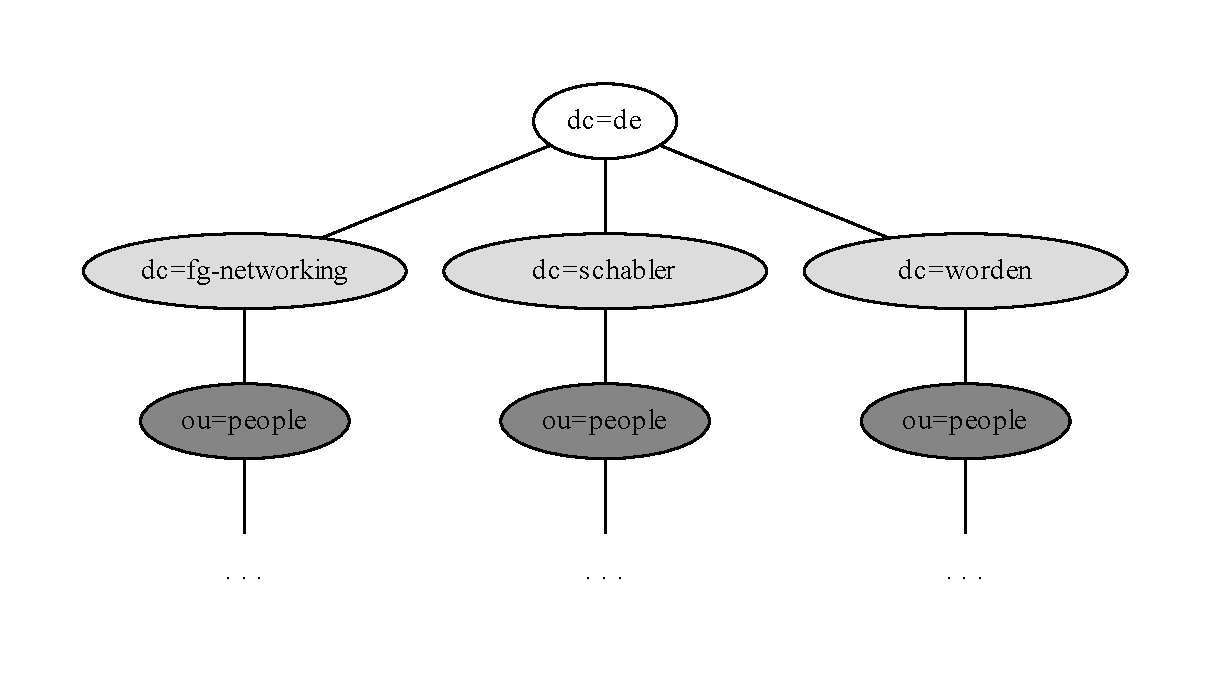
\includegraphics[width=\textwidth]{LDAP-fgn.pdf}
\caption{Der fertige LDAP-Verzeichnibaum}
\label{fig:LDAP-Baum}
\end{figure}

\subsubsection{Installation und Konfiguration des RADIUS-Servers}\label{sec:RADIUS-Konf}
Auf dem Server wurden die Pakete \texttt{freeradius} und \texttt{freeradius-ldap} sowie -- zu Testzwecken -- das Paket \texttt{freeradius-utils} installiert. In den Konfigurationsdateien wurde dann LDAP als mögliche Quelle für Benutzerdaten eingetragen, die LDAP-Module aktiviert und der Zugriff durch die E-Mail-Server der TU Kaiserslautern erlaubt. Zusätzlich musste das zu dem TU E-Mail-Servern gehörende Shared Secret eingetragen werden, welches aus den Konfigurationsdateien von CommuniGate übernommen wurde, da es nicht in der firmeninternen Dokumentation festgehalten war. Näheres zur Konfiguration siehe \autoref{sec:RADIUS-Konfig}

\subsubsection{Absicherung des Rechners (Firewall etc.)}
Wie in \nameref{sec:Sicherheitskonzept} erläutert, sind dem Netz in dem sich der Server befindet bereits zwei Firewalls vorgeschaltet. Die einzige Änderung, die an diesen vorgenommen werden musste ist das Eintragen einer Ausnahmeregel mit der der Zugriff auf den RADIUS-Server aus dem Universitätsnetz erlaubt wird. Dafür wird die bereits bestehende Firewall-Regel für den in CommuniGate enthaltenen RADIUS auf die IP des neuen Servers angepasst.

Zusätzlich zu den Firewalls, die bereits das Firmennetz der fgn GmbH schützen, wurde die simpel zu bedienende Uncomplicated Firewall (\texttt{ufw}) verwendet, um lediglich die für OpenLDAP, FreeRADIUS und SSH notwendigen Ports zuzulassen, und Netzwerkverbindungen auf den restlichen Ports nicht zuzulassen. Näheres zur Firewall Konfiguration siehe \autoref{sec:Firewall-Konfig}.

Der OpenLDAP-Server wurde so konfiguriert, dass er lediglich SSL verschlüsselte Verbindungen zulässt, somit ist ein Abhören der Kommunikation mit dem LDAP-Server stark erschwert. Modifikation der Daten im Verzeichnisdienst ist nur dem LDAP-Administrator-Benutzer gestattet, der mit einem -- den Passwortrichtlinien von fgn entsprechenden -- Passwort gesichert ist. Die Firewall auf dem Server lässt außerdem nur Verbindungen aus dem Firmennetz und nur auf dem entsprechenden Port (636) zu. Als anonymer Benutzer ist lediglich der Zugriff auf Attribute, die nur anderweitig öffentlich verfügbare Informationen wie Name des Anwenders enthalten, und das Testen eines Passworts gegen den gespeicherten Passwort Hash. Letzteres wäre ein ernstzunehmender Angriffspunkt wenn Verbindungen zum LDAP-Server von außerhalb des Firmennetzes erlaubt wären, was aber durch die Firewalls verhindert wird.

Zum FreeRADIUS-Server können sich generell nur Clients verbinden, die vorher in die Konfiguration eingetragen wurden, da beide Seiten das Shared Secret einstellen müssen. Verbindungen von komplett unbekannten Clients können somit schon rein prinzipbedingt nicht aufgebaut werden. Der einzige Angriffsvektor in dieser Richtung ist also ein Client, der das Shared Secret zwischen dem FreeRADIUS und den TU E-Mail-Servern kennt. Leider ist das Shared Secret die große Schwachstelle des RADIUS-Protokolls (was auch seit ungefähr 15 Jahren hinlänglich bekannt ist), somit ist das Einzige das dagegen unternommen werden kann eine Verbindungsbeschränkungen z.B. durch eine Firewall. Die einzige Möglichkeit eines unberechtigten Zugriffs wäre danach das Herausfinden des Shared Secrets und das Spoofing der IP eines TU Kaiserslautern E-Mailservers. Beides zusammen genommen ist recht unwahrscheinlich und wird noch dadurch erschwert dass die TU selbst Maßnahmen gegen IP-Spoofing in dem von ihr verwalteten Netz (131.246.0.0/16) betreibt.

Der OpenSSH-Server, der für Fernzugriffe zusätzlich zur eigentliche Serverfunktion auf dem Rechner läuft, wird mit der Debian Standardkonfiguration betrieben unter denen Zugriff auf den root-Account nur mit einem eingetragenen SSH-Key möglich ist. Es existieren auch keine normalen Benutzerkonten auf dem Rechner, weswegen das Angriffsszenario vom Kapern eines Benutzeraccounts und dem darauffolgendem Erlangen von root-Rechten durch eine Schwachstelle (Priviledge Escalation) ausfällt. Wie bei sämtlichen fgn-Servern wurde der SSH-Zugang aus dem gesamten Internet erlaubt. Hier werden aber Brute-Force- Attacken durch die fgn-Firewall erschwert da diese für SSH-Verbindungsversuche einen Rate Limiter eingestellt hat.

%\hilight{TODO: fgn Netzstruktur korrigieren}

\subsection{Abschließende Arbeiten}
\subsubsection{Umkonfiguration der Webservices}
Da die umzustellenden Dienste (Webservices und OpenVPN) bereits den alten LDAP-Server verwenden, musste hier nicht viel eingerichtet werden. Die größte Änderung, die vorzunehmen war, ist daher das zusätzliche Eintragen des CA-Stammzertifikates in die Konfigurationsdatei \texttt{/etc/apache2/mods-available/ldap.conf} (bzw. bei OpenVPN in die entsprechende Konfigurationsdatei), da sonst keine LDAP- Verbindung über SSL aufgebaut werden kann. Ansonsten mussten nur noch in der Site-Konfiguration die URL des LDAP Servers und die BaseDN angepasst werden (OpenVPN ist analog anzupassen). Zu Details der anzupassenden Konfigurationen siehe \autoref{sec:Apache-Konfig} und \autoref{sec:VPN-Konfig}.

Wie in \nameref{sec:Konfig-Doku-Alt} geschildert, konnte Egroupware zur Bearbeitungszeit dieses Projektes noch nicht umgestellt werden, dies muss dann noch vom zuständigen Mitarbeiter vorgenommen werden.

\subsubsection{Import/Anlegen der Anwenderkonten}
Wie in \nameref{sec:Importsuche}) erwähnt, wurde entschieden, dass die praktikabelste Methode, um die Benutzerkonten im neuen Verzeichnisdienst zu erstellen, die Generierung einer von LDAP importierbaren Datei ist. Mit Hilfe der von Herrn Auerswald erstellten Skripte (Skripte siehe \autoref{sec:SkriptA} und \autoref{sec:SkriptB}) wurde dann aus den Daten von CommuniGate eine LDIF-Datei erzeugt, die dann mit \texttt{ldapadd} importiert wurde.

Anmerkung: CommuniGate speichert Mailinglisten und Ähnliches ebenfalls in LDAP-Objekten, es wurden hier nur die Konten von echten Anwendern und zur Verwaltung der Webservices etc. nötige Konten importiert.

\subsubsection{Funktions- und Sicherheitstests}
Schon während der Arbeiten wurden immer wieder prüfbare Teilkomponenten getestet: 
Vor dem Erstellen der Verzeichnisstruktur wurde bereits eine Teststruktur erstellt, die lediglich die \texttt{fg-networking}-Domain und ein Testkonto enthielt. Dieses Testkonto wurde dann mit Hilfe von \texttt{ldapsearch} aus den LDAP-Utils abgefragt, noch bevor LDAPS eingerichtet war. Nach der Einrichtung von LDAPS wurde das Stammzertifikat in die Konfigurationsdatei \texttt{/etc/ldap/ldap.conf} eingetragen auf den Rechnern, auf denen mit den LDAP-Utils getestet wurde. Dies ist aber für den Normalbetrieb nicht notwendig da dieser Eintrag nur von den LDAP-Utils ausgewertet wird. Apache und OpenVPN haben dazu eigene Einstellungen.

Die Webservices auf \texttt{nms} wurden dann kurzzeitig auf dieses LDAP umgestellt, um die generelle Funktion der Authentifizierung testen zu können. Der Rechner \texttt{nms} wurde gewählt, da die Webservices auf ihm wenig benutzt werden, und das auch nur von Mitarbeitern, die zur Bearbeitungszeit vor Ort waren und so einfach und schnell über die Tests informiert werden konnten. Hierbei fiel auf, dass es anfänglich noch einen Fehler in den SSL-Einstellungen gab. Dieser stellte sich aber aber nach kurzer Fehlersuche als ein einfacher Tippfehler in der Apache-Konfiguration heraus. Nach Korrektur dessen konnte man sich mit dem Testkonto erfolgreich an den Webservices anmelden.

Die Anbindung des FreeRADIUS-Servers an den OpenLDAP-Server wurden mit Hilfe des Programms \texttt{radtest} aus den FreeRADIUS-Utils getestet. Hier wurde -- unter Verwendung des Shared Secrets -- das oben erwähnte Testkonto abgefragt. Mit demselben Befehl, aber einem echten Anwenderkonto, wurde auch der CommuniGate-Server getestet um einen Vergleichswert zu haben, da ein echter Praxistest erst bei Fertigstellung des neuen E-Mail-Servers durchgeführt werden kann.

Abschließend wurde noch versucht einen Managed Switch an den RADIUS-Server anzubinden, damit darüber Benutzerkonten aus dem LDAP-Verzeichnisdienst zum Anmelden verwendet werden können. Nach Informationen aus den LDAP-Logs funktionierte das Authentifizieren am Server auch, allerdings konnte man sich trotzdem nicht erfolgreich am Switch anmelden. Dafür hätte man zusätzliche Berechtigungen im LDAP hinterlegen müssen. Da nicht sofort ersichtlich wurde, was genau dafür zu konfigurieren wäre, und die Anbindung von Switches erst irgendwann in Zukunft geschehen soll, wurde das Ganze dann nicht weiter verfolgt.

\medskip \noindent
Zum Testen der Sicherungsmaßnahmen wurde nach der Umstellung der Webservices erfolglos versucht sich an diesen mit falschen Anmeldeinformationen (falscher Benutzername, richtiger Benutzername mit falschem Passwort) anzumelden. Dasselbe wurde mit \texttt{radtest} am RADIUS-Server getestet.
Abschließend wurde noch per \texttt{nmap} von innerhalb der Firmennetze und von einem externen Rechner aus geprüft, ob ausschließlich die richtigen Ports geöffnet sind (näheres dazu in \autoref{sec:NMAP-Test-int} und \autoref{sec:NMAP-Test-ext}).
%\hilight{TODO: fgn Netzstruktur korrigieren}


\section{Projektkosten}\label{sec:Kosten}
\begin{tabularx}{\textwidth}{|X|r|r|r|}
\hline
\mcc{4}{Kosten für die Einrichtung}\\
\hline
Kosten-Kategorie	&	Projekt &	CommuniGate-Upgrade &	keine Änderung\\
\hline
Hardware &	0,00\euro{} &	0,00\euro{} &	0,00\euro{}\\
\hline
Softwarelizenzen &	0,00\euro{} &	1.849,00\euro{} &	0,00\euro{}\\
\hline
Arbeitsaufwand &	2.485,00\euro{} &	2.485,00\euro{} &	0,00\euro{}\\
\hhline{|=|=|=|=|}
Gesamt &	2.485,00\euro{} &	4.334,00\euro{} &	0,00\euro{}\\
\hline
\end{tabularx}

\medskip \noindent Anmerkungen: Es wurde ein Stundenlohn von 71\euro{} angenommen. Hardwarekosten entstehen keine da alles auf Virtual Machines läuft und die Anschaffungskosten für die ESXi-Server nur schwierig auf die VMs aufzuteilen ist. Die Zusammensetzung der beiden Vergleichskostensätze findet sich in der \nameref{sec:Erwin}.

\bigskip\noindent
\begin{tabularx}{\textwidth}{|X|r|r|r|}
\hline
\mcc{4}{Jährliche Kosten}\\
\hline
Kategorie	&	Projekt &	CommuniGate-Upgrade &	keine Änderung\\
\hline
Hardware &	0,00\euro{} &	0,00\euro{} &	0,00\euro{}\\
\hline
Softwarelizenzen &	0,00\euro{} &	332,82\euro{} &	0,00\euro{}\\
\hline
Arbeitsaufwand &	355,00\euro{} &	213,00\euro{} &	2.350,00\euro{}\\
\hhline{|=|=|=|=|}
Gesamt &	355,00\euro{} &	545,82\euro{} &	2.350,00\euro{}\\
\hline
\end{tabularx}

\medskip \noindent Anmerkungen: Der Wartungsaufwand für das Projektsystem wurde auf fünf Stunden pro Jahr geschätzt, der für einen neuen CommuniGate Server nur auf drei Stunden da Unterstützung durch den professionellen Support von CommuniGate in den Lizenzkosten enthalten ist.

\section{Projektabschluss}
\subsection{Fazit}
Bis auf das Egroupware und der E-Mail-Server, wurden alle Systeme von fgn, die vorher den LDAP-Server von CommuniGate benutzten, erfolgreich auf den neuen OpenLDAP Server umgestellt. Da der alte E-Mail-Server weiterhin in Betrieb bleibt bis er vom neuen Server abgelöst wird findet bis dahin ein Parallelbetrieb der LDAP Server statt. Deswegen werden die Benutzerpasswörter bei Fertigstellung des neuen E-Mail-Servers noch einmal zur Sicherheit synchronisiert werden müssen, dies wird jedoch über die Skripte wieder einfach zu bewerkstelligen sein. Die im Rahmen dieses Projekts erstellten Skripte werden dazu allerdings leicht modifiziert werden müssen da diesmal LDAP Daten verändert werden sollen statt neu hinzugefügt, und die LDIF-Syntax dafür leicht anders ist.

Der FreeRADIUS-Server wurde ebenso erfolgreich eingerichtet und einfacher als erwartet an den OpenLDAP-Server angebunden. Allerdings verrichtet er bisher noch keinen sinnvollen Dienst, da bei fgn RADIUS momentan nur über den E-Mail-Server benutzt wird und dieser weiterhin selbst einen RADIUS-Server betreibt. Dies wird sich voraussichtlich erst mit der Fertigstellung des neuen E-Mail-Servers ändern.

Bei der Zeitplanung des Projektes wäre im Nachhinein Folgendes zu verbessern gewesen: Für den Entwurf und die Implementierung der Verzeichnisstruktur hätte mehr Zeit eingeplant werden müssen. Als der Zeitplan für den Projektantrag ausgearbeitet wurde, waren die Vorrecherchen zu LDAP und vor Allem zur bestehenden Konfiguration noch nicht weit genug fortgeschritten, dass Probleme aus dieser Richtung vorhersehbar gewesen wären. Insgesamt wäre der Entwurf der LDAP Verzeichnisstruktur am Besten als zusätzlicher Punkt zur Planung hinzugefügt worden. In der Umsetzungsphase hätte man dagegen weniger Zeit für die Vorbereitung veranschlagen können, da nur eine übersichtlich kleine Anzahl an Diensten den LDAP-Server verwendet und bei diesen nicht viel an der Konfiguration zu ändern war.

\subsection{Ausblick}
Die voraussichtliche erste Änderung -- nach der Anbindung von Egroupware -- für die im Rahmen dieses Projektes erstellten Serverdienste wird nach aktueller Planung die Anbindung des neuen E-Mail-Servers sein. Dafür werden den in OpenLDAP bestehenden Benutzerkonten die Attribute, die der E-Mail-Server benötigt (wie z.B. die E-Mailadresse), mit den korrekten Werten gefüllt werden müssen. Dies wird voraussichtlich wieder über durch Skripte erstellte LDIF-Dateien geschehen.

Ebenso bietet sich für eine Erweiterung des Projektsystems die Einbindung der anderen Linux-Rechner in der Firma an. Dort könnte man dadurch die bisherigen lokalen Benutzerkonten durch zentral in LDAP abgelegte und verwaltete Konten ersetzen. Dazu müsste man auf den Linux-Rechnern LDAP an das PAM-System anbinden (dazu müsste dort vermutlich noch ein passendes PAM-LDAP Modul installiert werden und eventuell auch das LDAP Modul für den Name Switch Service (\texttt{NSS})) und im LDAP-Server die Benutzer um die passenden Attribute (wie z.B. Home-Verzeichnis, UID, Gruppen) erweitern. Letzteres kann wieder geskriptet werden. Als Anwendersystem wird im Moment allerdings nur ein Rechner verwendet, und zwar \texttt{fgnfs}, für den der Aufwand im Vergleich zum zu erwartenden Nutzen im Rahmen des Projektes zu groß erschien.

Eine weitere für fgn attraktive Erweiterungsmöglichkeit ist das Anbinden der Managed Switches der Schulungslabore an den FreeRADIUS-Server (und somit an LDAP). Dies würde Problemen, die abundzu durch Änderungen der Anmeldeinformationen der Switches durch Schulungsteilnehmer auftreten, vorbeugen. Da die Schulungslabore in einem VPN sind müsste RADIUS dazu ebenfalls ins VPN gehängt werden. Desweiteren müssten Konten für die Switches erstellt werden, die die Attributen enthalten, die zu Autorisierung benötigt werden. In die Switches müsste außerdem der RADIUS-Server eingetragen und im RADIUS-Server die Clients eingetragen werden (jeweils dann mit passenden Shared Secret "Paaren").

fgn hat neben den diversen Linux-Rechnern auch noch 2 Windows-PCs in der Verwaltung, sowie einige an den Schulungslaboren angeschlossene virtuelle Windows-Rechner. Für diese könnte man mit Samba 4 eine kleine Active Directory-Domäne aufbauen die an den OpenLDAP Server angebunden wird. Allerdings benötigt Samba 4 inzwischen ein eigenes LDAP (dies wird für Replikationsfunktionen benötigt) und lässt sich somit nur umständlich an das nun bestehende LDAP anbinden. Dieser Erweiterungsmöglichkeit stellt -- von den bisher genannten -- für fgn die unattraktivste dar, da der Aufwand recht hoch wäre und es nur wenige Windowsrechner gibt die davon tatsächlich profitieren würden.

\newpage
\section*{Quellen}
\addcontentsline{toc}{section}{Quellen}
\hilight{TODO: Quellen auflisten}

\appendix
\newpage
\addcontentsline{toc}{section}{Anhänge} %fügt Überschrift Anhänge in die TOC ein
\section{Übernommene LDAP Attribute} \label{sec:LDAP-Attribute}
\begin{itemize}
\item\texttt{uid}: User ID, Name des Anwenderkontos
\item\texttt{sn}: SurName, Nachname des Anwenders
\item\texttt{givenName}: Vorname des Anwenders
\item\texttt{cn}: CommonName, voller Name des Anwenders
\item\texttt{displayName}: anzuzeigender Name des Anwenders
\item\texttt{userPassword}: Passwort des Anwenders (wurde mit \texttt{slappasswd} gehashed)
\end{itemize}

\newpage
\section{Erklärung der OpenLDAP Loglevel} \label{sec:LDAP-Loglevel}
\begin{tabularx}{\textwidth}{|c|l|X|}
\hline
Level &	Keyword &	Description\\
\hline
-1 &	any &	enable all debugging\\
\hline
0 &	  &	no debugging\\
\hline
1 &	(0x1 trace) &	trace function calls\\
\hline
2 &	(0x2 packets) &	debug packet handling\\
\hline
4 &	(0x4 args) &	heavy trace debugging\\
\hline
8 &	(0x8 conns)& 	connection management\\
\hline
16 &	(0x10 BER) & 	print out packets sent and received\\
\hline
32 &	(0x20 filter) &	search filter processing\\
\hline
64 &	(0x40 config) &	configuration processing\\
\hline
128 &	(0x80 ACL) &	access control list processing\\
\hline
256 &	(0x100 stats) &	stats log connections/operations/results\\
\hline
512 &	(0x200 stats2) &	stats log entries sent\\
\hline
1024 &	(0x400 shell) &	print communication with shell backends\\
\hline
2048 &	(0x800 parse) &	print entry parsing debugging\\
\hline
16384 &	(0x4000 sync) &	syncrepl consumer processing\\
\hline
32768 &	(0x8000 none) &	only messages that get logged whatever log level is set \\
\hline
\end{tabularx}
\noindent Quelle: \url{http://www.openldap.org/doc/admin24/runningslapd.html}

\noindent\hilight{TODO: Übersetzung der Log Erklärung}

\newpage
\section{Erläuterungen zu den verwendeten LDAP Schemas}\label{sec:LDAP-Schema}
\begin{enumerate}
\setcounter{enumi}{-1}
\item \texttt{core} -- Enthält LDAP Core Attribute (X.501), wird immer benötigt
\item \texttt{cosine} -- Enthält die LDAPv3 Attribute (Cosine and Internet X.500 (RFC1274))
\item \texttt{nis} -- Schema zur Verwendung von NIS, bei uns vermutlich nicht benötigt aber Teil der Linux/Unix Standardinstallationen
\item \texttt{inetorgperson} -- Schema für die gängigen Personenattribute und andere Attribute für organisationsorientierte Dienste
\item \texttt{freeradius} -- Schema für RADIUS Atrribute, aus der FreeRADIUS Doku (\texttt{/usr/""share/""doc/""freeradius/""examples/""openldap"".schema})
\item \texttt{postfix} -- Schema mit zusätzlichen Attributen für postfix address rewrite, von den Autoren des Galileo Press OpenLDAP 2.4 Praxisbuches (in der FGN Bibliothek)
\end{enumerate}
(0-3 sind Teil der Debian Standardkonfig)

\newpage
\section{Erstellung der Verzeichnisstruktur}\label{sec:Erstelle-DB}
Die leere Datenbank wurde mit dem interaktiven Debian config script (aufgerufen mit \texttt{dpkg-reconfigure slapd}) erzeugt. Als Domain und Organization Name wurde \texttt{de} genommen. Die restlichen Fragen wurden mit den Standardantworten beantwortet. Für die drei Domains wurde dann folgende LDIF-Datei (\texttt{add\_DNs.ldif}) zum Erzeugen verwendet
\begin{lstlisting}
dn: dc=fg-networking,dc=de
o: fg-networking.de
objectClass: top
objectClass: dcObject
objectClass: organization

dn: dc=schabler,dc=de
o: schabler.de
objectClass: top
objectClass: dcObject
objectClass: organization

dn: dc=worden,dc=de
o: worden.de
objectClass: top
objectClass: dcObject
objectClass: organization

\end{lstlisting}
Diese wird (nachdem man den LDAP daemon slapd gestoppt hat) in die Datenbank eingefügt mit
\begin{lstlisting}
slapadd -n 1 -l add_DNs.ldif
\end{lstlisting}
(Der Content wird hier mit \texttt{slapadd} eingefügt da dies der einfachste Weg ist um dcObjects in der LDAP Datenbank zu erstellen. Für die meisten anderen Datenmanipulationen ist ldapmodify die sicherere und sauberere Variante). Danach kann (und muss man für den nächsten Schritt auch) man \texttt{slapd} wieder starten.

Als nächstes wurden die \texttt{people} organizationalUnits erzeugt, in die alle User Einträge kommen sollen (da wir vor der Fertigstellung des neuen Mailservers nur echte Anwenderaccounts migrieren (keine Mailinglisten Accounts u.ä.) ist dies auch erstmal die einzige benötigte OU). Zum Erzeugen der OUs wurde wieder eine LDIF Datei (\texttt{add\_content.ldif}) erstellt.
\begin{lstlisting}
dn: ou=people,dc=fg-networking,dc=de
objectClass: organizationalUnit
ou: people

dn: ou=people,dc=schabler,dc=de
objectClass: organizationalUnit
ou: people

dn: ou=people,dc=worden,dc=de
objectClass: organizationalUnit
ou: people
\end{lstlisting}
Die wurde dann in die Datenbank eingefügt mit
\begin{lstlisting}
ldapmodify -a -H ldapi:/// -D cn=admin,dc=de -W -f add_content.ldif
\end{lstlisting}
Anschließend kann man die User einfügen. Wir haben dazu nach dem folgenden minimalem Template per Skript aus den Klartextdateien von CommuniGate das LDIF dafür generiert.
\begin{lstlisting}
dn: uid=username,ou=people,dc=fg-networking,dc=de
objectClass: inetOrgPerson
objectClass: person
uid: username
sn: Nachname
givenName: Vorname
cn: Vorname Nachname
displayName: Vorname Nachname
userPassword: password
\end{lstlisting}

\newpage
\section{Skript zum Auslesen der Anwenderkonten aus der CommuniGate Dateien}\label{sec:SkriptA}
\lstinputlisting[language=sh]{cg_accounts_to_ldap.sh}
\hilight{TODO: Erklärung}

\newpage
\section{Skript zum Hashen der Anwenderpasswörter}\label{sec:SkriptB}
\lstinputlisting[language=sh]{hash_passwords.sh}
\hilight{TODO: Erklärung}

\newpage
\section{Konfiguration des FreeRADIUS Servers}\label{sec:RADIUS-Konfig}
Zuerst einmal zusätzlich das Paket \texttt{freeradius-ldap} installieren (bei Debian sind zwar schon Beispielkonfigs für LDAP mitgeliefert, aber die tatsächlichen Module sind erst in diesem Paket enthalten). In \texttt{/etc/freeradius/clients.conf} muss unter \texttt{secret} das zu den Uni Mailservern passende Shared Secret eingetragen werden (dies wurde aus der Konfiguration von CommuniGate ausgelesen). Wenn noch Clients an den RADIUS angebunden werden sollen muss unten für die passenden IPs ein Shared Secret vergeben werden das dann auch im Client eingetragen werden muss.

Um LDAP als Authentifizierungsmethode für User zu aktivieren muss in \texttt{/etc/""free""radius/""users} folgende Zeile eingetragen werden:
\begin{lstlisting}
DEFAULT Auth-Type := LDAP
\end{lstlisting}
Hier ist zu beachten das \textbf{EAP nicht mehr funktioniert}. Soll EAP irgendwann benutzt werden sollen muss hier eine andere Möglichkeit gefunden werden (die Dokumentation schlägt eine ähnliche Eintragung für jeden Benutzer einzeln vor).

In \texttt{/etc/freeradius/modules/ldap} muss unter \texttt{server} der richtige LDAP Server (\texttt{id.""fg-networking.""de}) und unter \texttt{basedn} die richtige Searchbase angegeben werden (hier \texttt{dc=fg-networking,""dc=de}, \textbf{muss evtl. noch angepasst werden})

In \texttt{/etc/freeradius/sites-enabled/default} müssen alle Zeilen die \texttt{ldap} einkommentiert werden. Einzige Ausnahme bildet die Zeile bei der in den Kommentaren davor erwähnt das sie nur benötigt wird wenn \texttt{edir\_account\_policy\_check = yes} eingestellt wurde (Zeile 488 in der aktuellen Datei).

Zum Testen des Ganzen wurde \texttt{radtest} aus dem Paket \texttt{freeradius-utils} verwendet. Der Aufruf war:
\begin{lstlisting}
radtest <username> <passwort> id.fg-networking.de:1812 10	<shared-secret>
\end{lstlisting}
Die Werte in spitzen Klammern müssen natürlich durch die entsprechenden Werte ersetzt werden (ohne die spitzen Klammern).


\newpage
\section{Konfiguration der Firewall}\label{sec:Firewall-Konfig}
Der folgende Block zeigt die Ausgabe der Uncomplicated Firewall (\texttt{ufw}) über ihre aktuellen Regeln (\texttt{ufw} verwendet als Standardregel, die als letzte angewendet wird wenn keine andere Regel zutrifft, ein implizites \texttt{* DENY ALL} das nicht angezeigt wird):
\begin{lstlisting}
root@id:~# ufw status
Status: active

To                         Action      From
--                         ------      ----
22                         ALLOW       Anywhere
636                        ALLOW       131.246.197.0/25
636                        ALLOW       10.122.0.0/16
1812                       ALLOW       131.246.197.0/25
1813                       ALLOW       131.246.197.0/25
1812                       ALLOW       10.122.0.0/16
1813                       ALLOW       10.122.0.0/16
1812                       ALLOW       131.246.120.208/28
1812                       ALLOW       131.246.5.14
22                         ALLOW       Anywhere (v6)
\end{lstlisting}
\begin{itemize}
\item SSH (Port \texttt{22}) ist wie bei Servern bei fgn üblich von sämtlichen Quellrechnern erlaubt (IPv4 und IPv6)
\item LDAPS (Port \texttt{636}) ist aus dem fgn-Subnetz (\texttt{131.246.197.0/25}) und dem privaten Infrastruktur-Netz von fgn (\texttt{10.122.0.0/16})
\item RADIUS (Port \texttt{1812} ist der gerenelle Port des FreeRADIUS-Daemons und Port \texttt{1813} ist der Port für Accounting) sind zugelassen für Verbindungen aus dem fgn-Subnetz (\texttt{131.246.197.0/25}), dem privaten Infrastruktur-Netz von fgn (\texttt{10.122.0.0/16}), den TU E-Mail-Servern \texttt{131.246.120.208/28} und dem RADIUS-Server der TU \texttt{131.246.5.14}. Der RADIUS-Proxy Port \texttt{1814} wurde hier nicht gebraucht weswegen keine Verbindungen zu ihn friegeschaltet wurden.
\end{itemize}
Die Firewall-Regeln wurden nach Vorbild der Regeln für den CommuniGate Server erstellt.

\newpage
\section{Änderungen an der Apache Konfiguration}\label{sec:Apache-Konfig}
Zur Anbindung von LDAP an einen Apache Web-Server wird die \texttt{mod\_authnz\_ldap} verwendet. In der Konfig-Datei \texttt{/etc/apache2/mods-available/ldap.conf} muss auch wieder das CA Zertifikat eingetragen werden um LDAPS verwenden zu können. Dazu trägt man (außerhalb jeglichen \texttt{<Location>} Kontexts) ein:
\begin{lstlisting}
LDAPTrustedGlobalCert CA_BASE64 /etc/ssl/certs/fg-networking.de.pem
\end{lstlisting}
(In dieser Datei war bereits auch schon der ldap-status handler definiert, an dieser Einstellung muss nichts verändert werden). In der passenden Seitenkonfig (auf NMS: \texttt{/etc/apache2/sites-available/default-ssl}) muss man dann noch die URL vom LDAP Server anpassen. Auf NMS sieht die neue Konfig wie folgt aus:
\begin{lstlisting}
 <Location />
    AuthType  Basic
    AuthName  "FGN NMS"
    AuthzLDAPAuthoritative  off
    AuthBasicProvider ldap
    AuthLDAPURL ldaps://id.fg-networking.de:636/dc=fg-networking,dc=de?uid?sub?
    require valid-user
    Satisfy any
  </Location>
\end{lstlisting}

\newpage
\section{Änderungen an der OpenVPN Konfiguration}\label{sec:VPN-Konfig}
Konfigurationsdateien \texttt{/etc/openvpn/tcp.config} und \texttt{/etc/openvpn/udp.config}
\begin{lstlisting}
plugin /usr/lib/openvpn/openvpn-auth-ldap.so /etc/openvpn/auth-ldap.config
\end{lstlisting}
Die Einträge sind notwendig damit das LDAP Plugin überhaupt verwendet wird.

Konfigurationsdatei \texttt{/etc/openvpn/auth-ldap.config}
\begin{lstlisting}
<LDAP>
        URL             ldaps://id.fg-networking.de:636
        Timeout         15
        TLSEnable       no
        FollowReferrals yes
        TLSCACertFile   /etc/ssl/certs/fg-networking.de_ca.pem
</LDAP>

<Authorization>
        BaseDN          "dc=fg-networking,dc=de"
        SearchFilter    "(&(uid=%u))"
        RequireGroup    false
</Authorization>
\end{lstlisting}
OpenVPN muss neu gestartet werden, um die geänderte Konfigurationsdatei anzuwenden.

\newpage
\section{Ergebnis eines fgn internen NMAP Tests}\label{sec:NMAP-Test-int}
\hilight{TODO: Testlog einfügen und erläutern}
\newpage
\section{Ergebnis eines externen NMAP Tests}\label{sec:NMAP-Test-ext}
\hilight{TODO: Testlog einfügen und erläutern}
\newpage

%\nocite{*}
%\begin{thebibliography}{9}
%
%\bibitem{lamport94}
%  Leslie Lamport,
% \emph{\LaTeX: a document preparation system},
%  Addison Wesley, Massachusetts,
 % 2nd edition,
%  1994.
%
%\end{thebibliography}

\end{document}
